\documentclass[twocolumn]{article}
\usepackage{amsfonts}
\usepackage{amssymb}
\usepackage{amsmath}
\usepackage{tikz}
\usetikzlibrary{decorations.pathreplacing}
\usepackage{hyperref}
\hypersetup{
    colorlinks,
    citecolor=black,
    filecolor=black,
    linkcolor=black,
    urlcolor=black
}
\begin{document}

\title{Precourse SoM+SoED}
\author{Lecture notes by Rangi Siebert}
\maketitle
\tableofcontents

\section{Statements And Sets}
			\paragraph{Main Porpose of Mathematics:}
			Formulation of \textbf{Statements} and assessing weather certain 
			statements are \textbf{true (t,1)} or \textbf{false (f,0)} 

			\paragraph{Definition (informal):}
			A "statement" is an expression that is either true or false.

			\paragraph{Examples:}
			\begin{enumerate}
				\item "It is raining" is a statement
				\item "$x=5$" is a statement
				\item "The Navier-Stokes eq. have a unique solution in 
					three dimensions." is a statement.
			\end{enumerate}

	\subsection{Logical Connectives:}
		\textbf{Lofical connectives} combine / modify simple statements to 
		createnew ones. Main examples: Negation, And, Or, Implication, Equivalance

		\subsubsection{Negation}
			If $A$ is a statement, the $\neg A$ is the negation of $A$.\\
			It holds:
			\begin{enumerate}
				\item $\neg A$ is true if $A$ is false
				\item $\neg A$ is false if $A$ is true
			\end{enumerate}

%			\begin{table}[]
%			\begin{tabular}{l|l}
%				$A$ & $\neg A$ \\ \hline
%				0 & 1 \\
%				1 & 0
%				\end{tabular}
%			\end{table}

			\paragraph{Example:}
				$\neg(x=5)$ means $x\not=5$
			
		\subsubsection{And}
			If $A$ and $B$ are statements, then "$A\wedge B$" means "$A$ and $B$"
			\begin{enumerate}
			\item $A\wedge B$ is true if both $A$ and $B$ are true.
			\item $A\wedge B$ is false if at least one of the statements $A$ and $B$
				is false.
			\end{enumerate}
%			\begin{table}[]
%			\begin{tabular}{l|l|l}
%			$A$  & $B$  & $A\wedge B$  \\ \hline
%			0 & 0 & 0 \\
%			0 & 1 & 0 \\
%			1 & 0 & 0 \\
%			1 & 1 & 1 
%			\end{tabular}
%			\end{table}
			\paragraph{Example:}
				If $A$ is the statement "$x\le3$ " and $B$ the statement "$x$ 
				is a natural number", then $A\wedge B$ is "$x$ is 1, 2, or 3".

		\subsubsection{Or}
			If $A$ and $B$ are statements, then "$A\vee B$" means "$A$ or $B$".\\
			It holds:
			\begin{enumerate}
			\item $A\vee B$ is true if at least one of the statements $A$ and $B$ 
				is true
			\item $A\vee B$ is false if both the statements $A$ and $B$ are false	
			\end{enumerate}
			
			\paragraph{Note:}
				The "or" is not exclusive.

			\paragraph{Example:}
				If $A$ is the statement "$x$ is a natural number smaller than
				4" and $B$ is the statement "$x$ is a natural number greater
				 than 2", then $A\vee B$ is "$x$ is a natural number".

		\subsubsection{Implication}
			"$A\Rightarrow B$" means "If $A$ is true, then $B$ is true."
			\begin{enumerate}
			\item "$A\Rightarrow B$" means "if both $A$ and $B$ are true of if $A$ 
				is false"
			\item "$A\Rightarrow B$" is false, if $A$ is true and $B$ is false.	
			\end{enumerate}

			\paragraph{Example:}
				\[
				(\mbox{m, n}\in\mathbb N\wedge\mbox{m is even})
				\Rightarrow m*n \mbox{ is even}
				.\] 
			\paragraph{Proof:}
				Assume m, n are natural numbers. Then m is even
				\begin{itemize}%[leftmargin=1em]
				\renewcommand{\labelitemi}{$\Rightarrow$}
				\item $m=2*m'$ for some $m'\in\mathbb N$
				\item $m*n=2*m'*n$ with $m'\in\mathbb N$
				\item $m*n$ is even				
				\end{itemize}
			\paragraph{Note:}
				\[
					(A\Rightarrow B)\not\Rightarrow(B\rightarrow B)
				.\] 

		\subsubsection{Equivalance}
			"$A\Leftrightarrow B$" means "A is true if and only if B is true".\\
			It holds:
			\begin{enumerate}
			\item "$A\Leftrightarrow B$" is true if both $A$ and $B$ are true
				or if both $A$ and $B$ is false.
			\item "$A\Leftrightarrow B$" is false if $A$ is false and $B$
				is true or vice versa
			\end{enumerate}
			\paragraph{Note:}
				\begin{enumerate}
				\item ($(A\Leftrightarrow B)
					\Leftrightarrow
					\{(A\Rightarrow B)\wedge(B\Rightarrow A)\}$
				\item $(A\Rightarrow B)\Leftrightarrow(\neg B\Rightarrow\neg A)$ 
				\end{enumerate}
			\paragraph{Example:}
				For m, n natural numbers:
				\[
				m*n\mbox{ is even}\Leftrightarrow(\mbox{$m$ is even}\vee n\mbox{ is even})
				.\] 
			\paragraph{Proof:}
				Show:"$B\Rightarrow B$" and "$A\Rightarrow B$"
				\begin{enumerate}
				\item "$B\Rightarrow A$" is already proven; see above
				\item "$A\Rightarrow B$":\\
			 		We show the equvalent "$\neg B\Rightarrow\neg A$"\\
					Suppose $m$ is odd and $n$ is odd, i.e.,\\
					$m=2m'+1$, $n=2n'+1$, $m',n'\in\mathbb N_0$   
					\begin{itemize}%$ [leftmargin=1em]
					\renewcommand{\labelitemi}{$\Rightarrow$}
					\item $m*n=4m'n'+2(m’+n’)+1=2*k+1$; with $k:=2m’*n'+(m’+n’)\in\mathbb N_0$
				\item $m*n$ is odd 
					\end{itemize}
				\end{enumerate}

	\subsection{Quantifiers}
		Quantifiers describe quantitative properties:
		\begin{enumerate}
		\item $\forall$: for all
		\item $\exists$: exists
		\item $\exists_1$, $\exists!$: there exists precisely one
		\item $\not\exists$: there does not exist (i.e., $\neg\exists$)
		\end{enumerate}
			\paragraph{Example:}
				\[
				\forall x\in\mathbb R\exists n\in\mathbb N:n>x
				.\]
				\textbf{means:}\\
				"For all real numbers $x$, there exists a natural number
				$n$ such that $n$ is bigger than $x$" 
			\paragraph{Note:}
				The order matters

	\subsection{Sets}
			\paragraph{Definition (informal):}
				A collection of well-defined distinct objects is called a set.
				Teh objects contained in a set are called elements.
			\paragraph{Examples:}
				\begin{enumerate}
				\item The set of all countries on earth
				\item The set of all colors
				\end{enumerate}
			\paragraph{Description of Sets:}
				\begin{enumerate}
				\item Explicit definition(write all elements down)

					\[
					A=\{a,b,c,d\}
					.\]  
				\item Characterization by property
				\end{enumerate}
					\[
					A=\{\mbox{countries}\mid\mbox{contains the letter a}\}
					.\] 
					\[
					\mathbb Q:=\{x\in\mathbb R\mid\exists q\in\mathbb N
					:q*x\in\mathbb Z\} 
					.\] 

			\paragraph{Examples of Sets:}
				\begin{itemize}%[leftmargin=1em]
				\renewcommand{\labelitemi}{$\rightarrow$}
				\item $\mathbb N$ : natural numbers
				\item $\mathbb N_0$ : natural numbers and zero
				\item $\mathbb Z$ : integers
				\item $\mathbb Z$ : rational numbers
				\item $\mathbb R$ : real numbers 
				\item $\mathbb P$ : set of all prime numbers
				\item $\mathbb C$ : complex nubers
				\end{itemize}
			
			\paragraph{Def.: Intervals:}
				Let $a,b\in\mathbb R$. We define:
				\begin{itemize}%[leftmargin=1em]
				\renewcommand{\labelitemi}{$\rightarrow$}
				\item $[a,b]:=\{s\in\mathbb R\mid a\le s\le b\}$
				\item $(a,b]:=]a,b].=\{s\in\mathbb R\mid a<s\le b\}$ 
				\item $\mathbb R_{\ge0}:=[0,\inf)$
				\end{itemize}
	\subsection{Basic Set-Operations and Relations}
		\begin{itemize}%[leftmargin=1em]
		\renewcommand{\labelitemi}{$\rightarrow$}
		\item $a\in A$ : $a$ is an element of $A$ 
		\item $a\not\in A$ : $a$ is not an element of $A$ 
		\item $A\subset B$ : $A$ is a subset of $B$, i.e., $a\in A\Rightarrow a\in B$  
		\item $A\not\subset B$ : $A$ is not a subset of $B$,  
			$\exists a\in A:a\not\in B$
		\item $A\subsetneq B$ : $A$ is equal to $B$, i.e.,
			\[
			(A\subset B)\wedge(\exists b\in B:b\not\in A)
			.\] 
		\item $A=B$ : $A$ is equal to $B$, i.e., $(A\subset B)\wedge(B\subset A)$
		\item $A\cup B:=\{x\mid x\in A\vee x\in B\}$ (union)
		\item $A\cap B:=\{x\mid x\in A \wedge x\in B\}$ (intersection) 
		\item $A\backslash B=\{x\in A\mid x\not\in B\}$ ($A$ without $B$)
		\item $C_A(B):=A\backslash B$ in the situation $B\subset A$ 
		\item $\mid A\mid$ : the cardinality of $A$, i.e., number of elements
		\item $A\times B:=\{(a,b)\mid a\in A,b\in B\}$ Cartesian product of $A$ and $B$.
		\item $\emptyset$ : empty set
		\end{itemize}
			\paragraph{Example:}
				\[
				\emptyset <\mathbb P<\mathbb N<\mathbb N_0<\mathbb Z<
				\mathbb R<\mathbb C
				.\] 
			\paragraph{Note:}
				The operation $\cup$, $\cap$, $\times$ can be iterated.
				\[
				\bigcup_{i=1}^nA_i:=A_1\cup A_2\cup...\cup A_n,~n\in\mathbb N
				.\] 
				\[
				\bigcap_{i=1}^{n}A_i:=A_1\cap A_2\cap...\cap A_n,~n\in\mathbb N
				.\] 
				\[
				\prod_{i=1}^{n}A_1:=A_1\times A_2\times...\times A_n
				.\] 
			\paragraph{Example:}\mbox{}\\
				$A:=\{1,2,5,7\}$,   $B:=\{n\in\mathbb N\mid n\mbox{ is odd}\}$,
				\\
				$C:=\{2,\sqrt[]{2},B\}$,   $D:=\{1,5,7\}$ 
				\\\\
				$D\subsetneq B$, $D\subsetneq A$, $C\not\subset B$, 
				$B\in C$, $B\not\subset C$, $\{B\}\subset C$, 
				$B\backslash A=\{3\}\cup\{n\in\mathbb N\mid n\mbox{ is odd
				and }n\ge9\}$,\\
				
				\[
				\begin{split}
					C\times D=\{ & (2,1),(2,5),(2,7),\\
						     & (\sqrt[]{2},1),(\sqrt 2,5),(\sqrt2,7),\\
						     & (B,1),(B,5),(B,7)\}
				\end{split}
				\] 
				\[
				\mid C\times D\mid=9=\mid C\mid*\mid D\mid
				.\] 
		\subsubsection{Disjoint Sets}
			Two sets $A$ and $B$ are called disjoint if $A\cap B=\emptyset$ 
		
		\subsubsection{Calculus Rules for set operations:}
			If $A,B,C$ are sets, then it holds:
			\begin{enumerate}
			\item $A\cup B=B\cup A$, $A\cap B=B\cap A$ (commutativity)
			\item $A\cup(B\cup C)=(A\cup B)\cup C)$ \\
				$A\cap...$ (associativity)
			\item $A\cup(B\cap C)=(A\cup B)\cap(A\cup C)$\\
				$A\cap...$ (distributivity)
			\item $C\backslash(A\cap B)=(C\backslash A)\cup(C\backslash B)$\\
				$C\backslash(A\cup...$  (De Morgan)
			\item $\mid A\times B\mid=\mid A\mid*\mid B\mid$
			\item $\mid A\cup B\mid=\mid A\mid+\mid B\mid -\mid A\cap B\mid$
			\item $\mid A\backslash B\mid =\mid A\mid -\mid A\cap\mid $ 
			\end{enumerate}
			(5.-7. for $\mid A\mid,\mid B\mid<\inf$)

\section{Functions and Inequalities}
	\subsection{Functions}
		\paragraph{Definition:}
			Let $A$ and $B$ be nonempty sets. A function $f$ from $A$ to $B$ is 
			a rule that assigns to each element of the set $A$ a unique element 
			of the set $B$, i.e., 
			\[
			\forall x\in A\exists_1y\in B:y=f(x)
			.\] 
		
		\paragraph{Notation:}
			\[
			f:A\to B,x\mapsto f(x)
			.\] 
		
		\paragraph{Def.:}
			Let $f:A\to B$ be a function between nenempty sets $A$ and $B$. Then:
			\begin{itemize}%[leftmargin=1em]
			\renewcommand{\labelitemi}{$\rightarrow$}
			\item $A$ is called the domain.
			\item $B$ is called the codomain.
			\item The element $f(x)$ that a given $x\in A$ is mapped to by $f$ 
				is called the image of $x$ under $f$.
			\item For $C\subset A$, $f(C):=\{y\in B\mid \exists x\in C:f(x)=y\}$ 
			\item The set $\{(x,y)\in A\times B\mid y=f(x)\}$ is called the graph
				of $f$. 
			\end{itemize}
		\paragraph{Examples:}
			\begin{enumerate}
			\item If $A:=\{x\mid x\mbox{ is a mono-colored car}\}$ \\
				and $B:=set y\mid y\mbox{ is a color}$, then 
				\[
				f:=A\to B,~~f(x):=\mbox{color of }x
				.\] 
			\item If we consider for $A=\mathbb R$, the rule
				\[
					A\ni x\mapsto(-\inf,x]
				\]
				then this does not define a function 
				$f:\mathbb R\to\mathbb R $. But if we define the so-called
				power set of $\mathbb R $ by
				\[
				\mathbb P(\mathbb R ):=\{C\mid C\mbox{ is a subset of }
				\mathbb R \}
				,\]
				then $A\ni x\mapsto(-\inf,x]$ defines a function from 
				$\mathbb R $ to $\mathbb P(\mathbb R)$.
			\item The rule $g(x):=x^2$ defines a function whose domain and codomain
				is equal to $\mathbb R $, i.e., $g:\mathbb R\to\mathbb R,x
				\mapsto x^2$.
				\begin{itemize}%[leftmargin=1em]
				\renewcommand{\labelitemi}{$\rightarrow$}
				\item $g(\mathbb R )=[0,\inf)$ 
				\item For $C:=[-1,2]$ , $D:=[1,4]$:
					\[
						g(C)=[0,4]
					.\] 
				\end{itemize}
			\end{enumerate}
	
			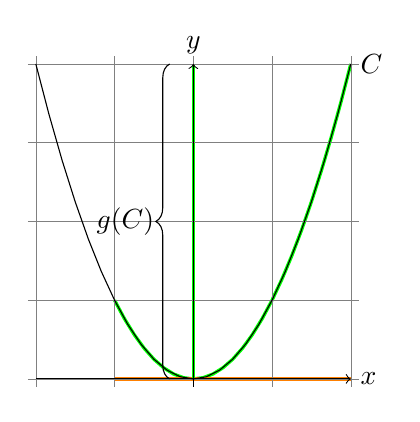
\begin{tikzpicture}[domain=-2:2]
			\draw[color=green,domain=-1:2,very thick] plot (\x,\x*\x) ;
			\draw[color=orange,very thick] (-1,0) -- (2,0);
			\draw[color=green,very thick] (0,0) -- (0,4);
			\draw[very thin,color=gray] (-2.1,-0.1) grid (2.1,4.1);
			\draw[->] (-2,0) -- (2,0) node[right] {$x$};
			\draw[->] (0,-.1) -- (0,4) node[above] {$y$};
			\draw[] plot (\x,\x*\x) node[right] {$C$};		
			\draw[decorate,decoration={brace,amplitude=5}]  (-0.3,0) -- (-0.3,4)
				node[midway,xshift=-16] {$g(C)$};
			\end{tikzpicture}

			\paragraph{Note:}
				In most applications the appearing functions are functions 
				between Euclidean spaces, i.e., $f:\mathbb R^n\to\mathbb R^m$,
				$n,m\in \mathbb N $

			\paragraph{Example:}
				\textbf{Minimize air resistance} \\
				Function from set of shapes to $\mathbb R $
		\subsection{Calculus Rules for Images and Preimages:}

			Let $f:A\to B$ be a map between nonempty sets $A$ and $B$. Then: 
			\begin{itemize}%[leftmargin=1em]
			\renewcommand{\labelitemi}{$\rightarrow$}
			\item $C_1\subset C_2\subset A\Rightarrow f(C_1)\subset f(C_2)$
			\item $D_1\subset D_2\subset B\Rightarrow f^{-1}(D_1)\subset f^{-1}
				(D_2)$
			\item $f(C_1\cup C_2)=f(C_1)\cup f(C_2)$,
				$\forall C_1,C_2\subset A$  
			\item $f^{-1}(C_1\cap D_2)=f^{-1}(D_1)\cup f^{-1}(D_2)$,   
				$\forall D_1,D_2\subset A$ 
			\item $f(C_1\cap C_2)\subset f(C_1)\cap f(C_2)$,   $\forall 
				C_1,C_2\subset A$ 
			\item $f^{-1}(D_1\cap D_2)=f^{-1}(D_1)\cap f^{-1}(D_2)$,   
				$\forall D_1,D_2\subset B$ 
			\item $C\subset f^{-1(f(C))}$,   $\forall C\subset A$\\
				ex.: $f:\mathbb R\to\mathbb R ,x\mapsto0\in\mathbb R $
				\begin{itemize}%[leftmargin=1em]
				\renewcommand{\labelitemi}{$\rightarrow$}
				\item C=\{0\}
				\item $f(C)=\{0\}$ 
				\item $ f^{-1}(f(C))=\mathbb R $ 
				\end{itemize}
			\item $f(f^{-1}(D))\subset D$,   $\forall D\subset B$   
			\end{itemize}
	\subsection{Mapping Properties}
		\subsubsection{Injectivity}
			Let $f:A\to B$ be a function between non-empty sets. 
			Then $f$ is called \textbf{injective} if:
			\[
			\forall x_1,x_2\in A,x_1 \not=x_2:f(x_1)\not=f(x_2)
			.\] 
		\subsubsection{Surjectivity}
			Let $f:A\to B$ be a function between non-empty sets. 
			Then $f$ is called \textbf{surjective} if:
			\[
			\forall y\in B\exists x\in A:f(x)=y
			.\] 
		\subsubsection{Bijectivity}
			Let $f:A\to B$ be a function between non-empty sets. 
			Then $f$ is called \textbf{bijective} if $f$ is injective and
			surjective,
			\[
			\forall y\in B\exists_1x\in A:f(x)=y
			.\] 
	
			\paragraph{Example:}
				The function $g(x):=x^2$ is nither surjective nor injective
				as a map from $\mathbb R $ to $\mathbb R $. However, $g$ is:
				\begin{itemize}%[leftmargin=1em]
				\renewcommand{\labelitemi}{$\rightarrow$}
				\item surjective as a map $g:\mathbb R \to[0,\inf)$
				\item bijective as a map $g:[0,\inf)\to[0,\inf)$ 
				\end{itemize}
				\textbf{$\Rightarrow$ choice of domain and co-domain crucial}
				

















\end{document}

